\section{Clustering}

	\section*{K-means clustering}

	{\bf You are given the one-dimensional data set shown in Table 2. Perform k-Means
	clustering on this data. Perform the clustering for two initial centroids: 2 and
	5; and for three initial centroids: 2, 6, 8. Document your observations.}

	\noindent\makebox[\linewidth]{\rule{\textwidth}{1pt}} 

	\begin{wraptable}{l}{3cm}
		\begin{tabular}{| p{1cm} | p{1cm} |}
			\hline
			{\bf ID} & {\bf X} \\ \hline
			P1 & 3 \\
			P2 & 1 \\
			P3 & 2 \\
			P4 & 4 \\
			P5 & 7 \\
			P6 & 9 \\
			P7 & 6 \\
			P8 & 9 \\
			P9 & 6 \\
			P10 & 8 \\ \hline
		\end{tabular}
		\caption{k-means}
	\end{wraptable}
	In this task we will use the k-means clustering algorithm to make 
	clustersf from the given inital points.
	The Algorithm starts with adding each point to the closest centroid. 
	After assigning the points
	to the closest centorid, we have what is called a cluster. A cluster is a 
	group of point that is assigned to a centroid. 
	When we have the initial clusters, we begin calculating the mean for each 
	cluster and see if we need to change the centroids and/or move points from
	one clutser to another cluster. 
	We are doing iterations until no points are changing cluster, and we have
	convergence. Clustering complete.
	In the first clustering we start with the initial centroids 2 and 5 (figure1).
	The red circle is centroid at X=2 and the blue is the centroid at X=5.
	We assigned P1-P3 to centroid 2, and P4-P10 to centroid 5.
	We now calculate the mean for each centroid to see if we can reassign any
	locations of centroid and points. If we calculate the mean for the cluster 
	with centroid X=2 we get (1 + 2 + 3)/3 = 2 and the mean for cluster X=5 we
	get (4 + 6 + 6 + 7 + 8 + 9 + 9)/7 = 7. 

	\begin{figure}[H]
		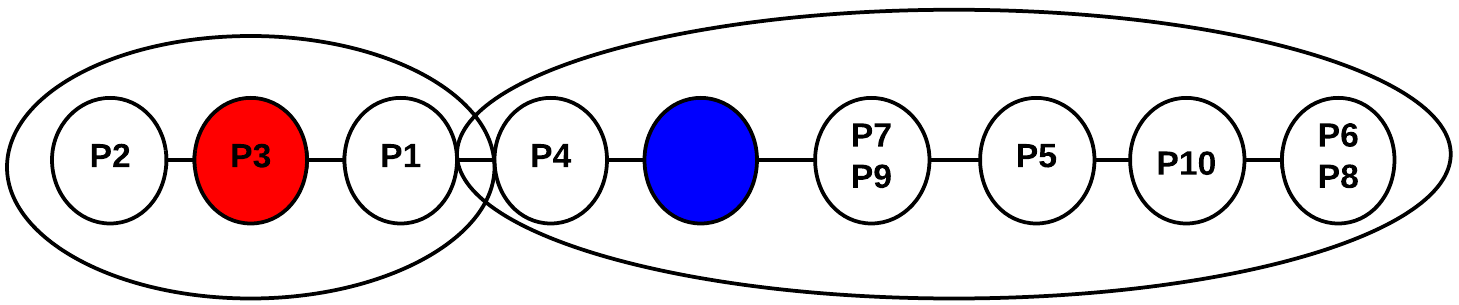
\includegraphics[width=\textwidth]{pics/clustering1.png}	
		\caption{Initial centroids 2 and 5}
	\end{figure}

	The results of the new centroids is that we reassigned some of the points
	as a result of the new positions of the centroids (figure2).

	\begin{figure}[H]
		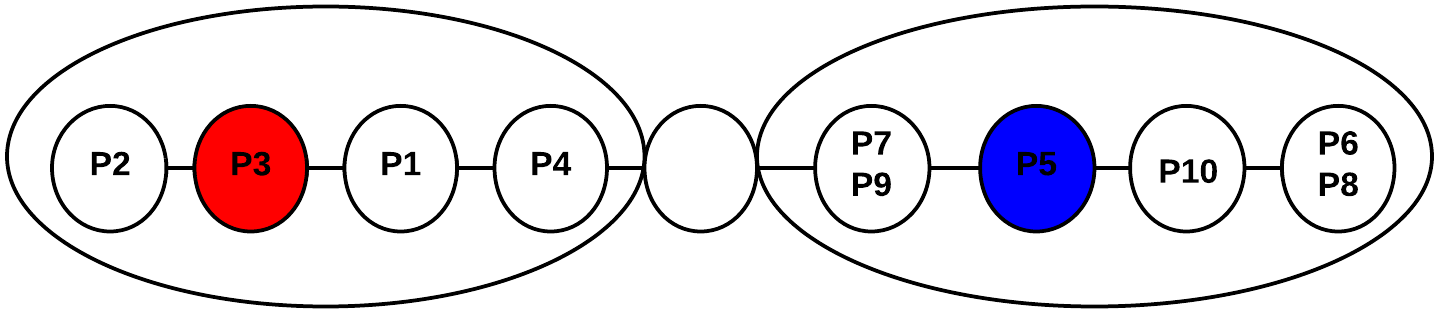
\includegraphics[width=\textwidth]{pics/clustering3.png}	
		\caption{Iteration 1}
	\end{figure}

	We still need to repeat the calculation until we get convergence. We now
	calculate the mean for the new clusters in figure 2. We then get the mean
	(1 + 2 + 3 + 4)/4 = 2.5 = 3 and (6 + 6 + 7 + 8 + 9 + 9)/6 = 7.5 = 8.
	The new clusters with the new centroids are showing in figure 3.


	\begin{figure}[H]
		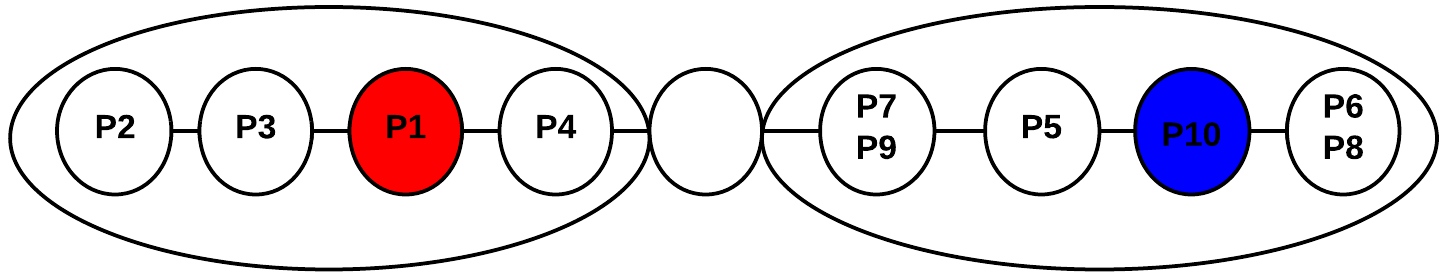
\includegraphics[width=\textwidth]{pics/clustering5.png}	
		\caption{Iteration 2}
	\end{figure}

	The result was that we moved the centroids, but no one of the point were
	reassigned. We can now say that the clustering is complete because the
	centroids will not move, and the points will not move. We have
	convergence. {\bf Clustering complete after 2 iterations}.

	\clearpage
	We will now use the same algorithm with the initial centroids 2, 6 and 8. 
	Figue 4 illustrate the clusters with the initial centroids. As we can see,
	there is many possible organizations of the clusters because some of the 
	points have the same distance to more than 1 centroid. In this assignment
	we use "add to the first and best". 

	\begin{figure}[H]
		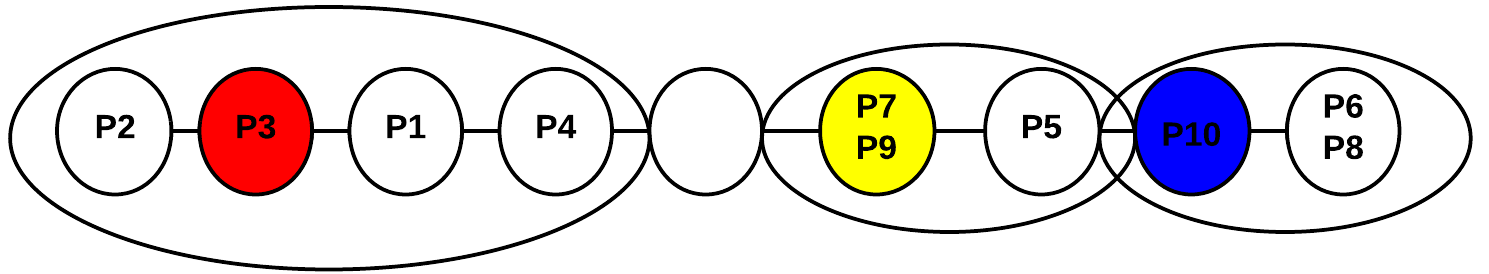
\includegraphics[width=\textwidth]{pics/clustering2.png}	
		\caption{K-means with centroids 2, 6 and 8}
	\end{figure}

	In the first iteration we calculate the mean of the clusters. The results is
	showing in figure 5. As we can see, we have moved the centroids from 2, 5, and 8 to 
	3, 6 and 9. No points changed their centroid. 

	\begin{figure}[H]
		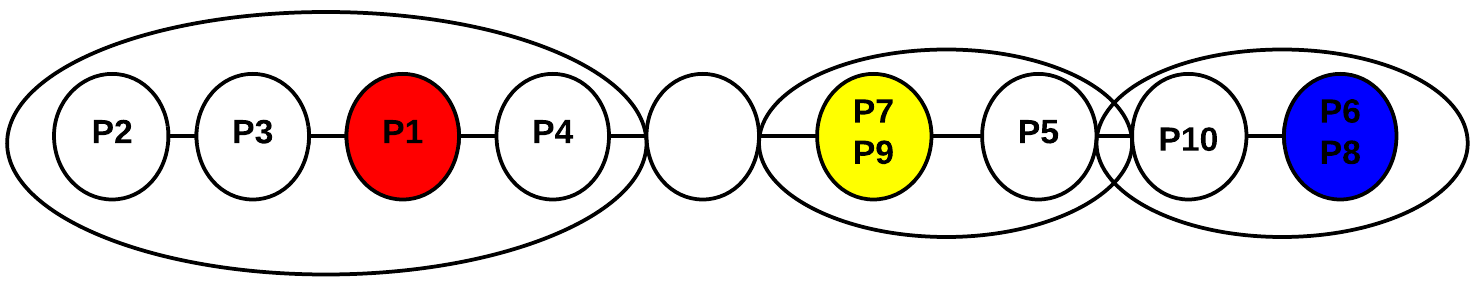
\includegraphics[width=\textwidth]{pics/clustering4.png}	
		\caption{Iteration 1}
	\end{figure}

	Can we do more iterations? There is no need of doing any more iterations because
	the centroids will not change because the mean remains the same. 
	We have convergence. {\bf Clustering complete after 1 iteration}.

	\clearpage
	\subsection{Hierarchical Agglomerative Clustering HAC}

		{\bf Explain the hierarchical clustering and the difference between MIN-link
		and MAX-link.}

		\noindent\makebox[\linewidth]{\rule{\textwidth}{1pt}} 

		{\bf Hierarchical clustering:} is a clustering method layers each clustering iteration.
		The iterations can start with points as individual clusters, and at each step, merge
		the closest pairs of clusters. We can also start with one, all-inclusive cluster and, 
		at each step, split the cluster into singleton clusters. For both methods, each
		iteration makes it own layer, a hierachy.

		{\bf MIN-link (single link):} defines cluster proximity as the proximity between the closest two points
		that are in different clusters (the shortest edgebetween two nodes in different subsets
		of nodes).

		{\bf MAX-link (complete link):} takes the proximity between the farthest two points in different clusters
		to be the cluster proximity (the longest edge between two nodes in different subsets of
		nodes).

		{\bf Difference between MIN-link and MAX-link:} the approach is mainly the same, only the
		definition of the distance is the difference, wr either define the distance ad max or min
		in each cluster.

		\clearpage

		{\bf Perform hierachical agglomerative clustering on the 2-dimentional dataset and
		show the resulting dendogram. Perform both MIN-link and MAX-link. Show all the 
		calculations. }

		\begin{table}[H]
			\centering
			\begin{tabular}{>{\centering\arraybackslash} p{1.5cm} | >{\centering\arraybackslash} p{1.5cm} | >{\centering\arraybackslash} p{1.5cm}}
				\hline
				{\bf Node ID} & {\bf X} & {\bf Y} \\ \hline
				1 & 1 & 11 \\
				2 & 1 & 9 \\
				3 & 1 & 5 \\
				4 & 1 & 2 \\
				5 & 6 & 7 \\
				6 & 11 & 7 \\ \hline
			\end{tabular}
			\caption{2-dimentional dataset for hierachical agglomerative clusering}
		\end{table}

		\noindent\makebox[\linewidth]{\rule{\textwidth}{1pt}} 

		In order to perfrom MIN-linking and MAX-linking, we need to calculate the distances
		of each coodinate point (x,y). The distance between two points a and b is defined by the 
		equation:

		\begin{equation}
			dist(a,b) = \sqrt{(X_{b} - X_{a})^{2} + (Y_{b} - Y_{a})^{2}}
		\end{equation} 

		\begin{table}[H]
			\begin{tabular}{ c | c | c | c | c | c | c | c }
				{\bf a} & {\bf b} & {\bf $X_{a}$} & {\bf $X_{b}$} & {\bf $Y_{a}$} & {\bf $Y_{b}$} 
				& {\bf Calculations} & {\bf Distance} \\ \hline
				1 & 2 & 1 & 1 & 11 & 9 & $\sqrt{(1-1)^{2} + (9-11)^{2}}$ & 2 \\
				1 & 3 & 1 & 1 & 11 & 5 & $\sqrt{(1-1)^{2} + (5-11)^{2}}$ & 6 \\
				1 & 4 & 1 & 1 & 11 & 2 & $\sqrt{(1-1)^{2} + (2-11)^{2}}$ & 9 \\
				1 & 5 & 1 & 6 & 11 & 7 & $\sqrt{(6-1)^{2} + (7-11)^{2}}$ & 6.40 \\
				1 & 6 & 1 & 11 & 11 & 7 & $\sqrt{(11-1)^{2} + (7-11)^{2}}$ & 10.77 \\
				2 & 3 & 1 & 1 & 9 & 5 & $\sqrt{(1-1)^{2} + (5-9)^{2}}$ & 4 \\
				2 & 4 & 1 & 1 & 9 & 2 & $\sqrt{(1-1)^{2} + (2-9)^{2}}$ & 7 \\
				2 & 5 & 1 & 6 & 9 & 7 & $\sqrt{(6-1)^{2} + (7-9)^{2}}$ & 5.39 \\
				2 & 6 & 1 & 11 & 9 & 7 & $\sqrt{(11-1)^{2} + (7-9)^{2}}$ & 10.20 \\
				3 & 4 & 1 & 1 & 5 & 2 & $\sqrt{(1-1)^{2} + (2-5)^{2}}$ & 3 \\
				3 & 5 & 1 & 6 & 5 & 7 & $\sqrt{(6-1)^{2} + (7-5)^{2}}$ & 5.39 \\
				3 & 6 & 1 & 11 & 5 & 7 & $\sqrt{(11-1)^{2} + (7-5)^{2}}$ & 10.20\\
				4 & 5 & 1 & 6 & 2 & 7 & $\sqrt{(6-1)^{2} + (7-2)^{2}}$ & 7.07 \\
				4 & 6 & 1 & 11 & 2 & 7 & $\sqrt{(11-1)^{2} + (7-2)^{2}}$ & 11.20 \\
				5 & 6 & 6 & 11 & 7 & 7 & $\sqrt{(11-6)^{2} + (7-7)^{2}}$ & 5 \\ \hline
			\end{tabular}
		\end{table}

		On the next page, we will use the results from this table to do a hierachical 
		agglomerative clustering with both MIN and MAX linking.

		{\bf MIN-linking dendrogram:}
			\begin{enumerate}
				\item (1), (2), (3), (4), (5), (6)
				\item (1, 2), (3, 4), (5, 6)
				\item (1, 2, 3, 4), (5, 6)
				\item (1, 2 , 3, 4, 5, 6)
			\end{enumerate}

		{\bf MAX-linking dendrogram:}
			\begin{enumerate}
				\item (1), (2), (3), (4), (5), (6)
				\item (4, 6), (1,  5), (2, 3)
				\item (4, 6, 1, 5), (2, 3)
				\item (1, 2 , 3, 4, 5, 6)
			\end{enumerate}


 
	\clearpage
	\subsection{Clustering Methods}
		{\bf Given the following three descriptions of datasets, decide what clustering algorithm
		to use and argue why (i.e. for each of the datasets choose one of k-means, HAC, or DBSCAN).
		Further, assign one best-matching clustering algorithm to each data plot from figure 1. Explain
		what the advantages and disadvantages of the different algorithms are and why they fit
		the different kinds of data:}

		\noindent\makebox[\linewidth]{\rule{\textwidth}{1pt}} 

		\subsection*{Choose clustering algorithm}
		
		\begin{itemize}
			\item {\bf Text collection (100.000 documents, 30.000 dimensions/distinct words):}
			DBSCAN would fit this data set because it is good at locating regions of high density that
			are seperated from one another by regions of low density. 
			
			\item {\bf Noisy data collection (200 instances, 3 dimensions):}

			\item {\bf Data collection with only little noise, with taxonimy-like relations in 
			between some of the instances (ca 400 instances, around 20 dimensions):}

		\end{itemize}

		\noindent\makebox[\linewidth]{\rule{\textwidth}{1pt}} 

		\subsection*{Assign clustering algorithm to data plot}


